\documentclass[oneside,final,14pt]{extreport}
\usepackage[utf8]{inputenc}
\usepackage[russianb]{babel}
\usepackage{vmargin}
\usepackage{amsmath}
\usepackage{amsfonts}
\usepackage{amssymb}
\usepackage{graphicx}
\usepackage[usenames]{color}
\setpapersize{A4}
\setmarginsrb{2cm}{1.5cm}{1cm}{1.5cm}{0pt}{0mm}{0pt}{13mm}
\usepackage{indentfirst}
\sloppy



\begin{document}

\section* {
\begin{centering}
	Вычислительные Методы\\
	Отчёт по лабораторной работе №3\\
\end{centering}
}


\begin{center}
	Выполнил студент группы КЭ-201 Гордеев Александр\\
	Вариант № 8\\
	Метод Ньютона\\
\end{center}


\[
	\begin{cases}
		f(x, y) = x + 3(lgx)^2 - y = 0     \\
		g(x, y) = 2x^2 - xy - 5x + 1 = 0 \\
	\end{cases}
\]

$f'_x = 1 + 6 * \frac{\ln x}{x*(\ln 10)^2}$

$f'_y = -1$

$g'_x = 4*x - y - 5$

$g'_y = -x$

\begin{center}
	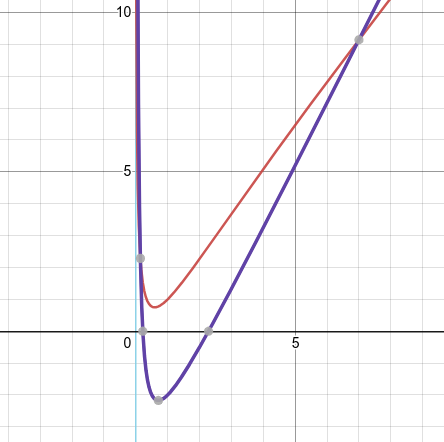
\includegraphics[scale=0.6]{lab3.png}

	По графику видны примерные точки:

	$x_{01} = 0.1$ 
	$y_{01} = 2$ \\
	$x_{02} = 7$
	$y_{02} = 9$ \\
\end{center}

Ответ, выданный программой:
\begin{center}
	$x_1 = 0.14286589, y_1 = 2.28530313$

	$x_2 = 6.99957134, y_2 = 9.14200858$
\end{center}

\end{document}
